\documentclass[12pt]{article}

\usepackage[english, greek]{babel}
\newcommand{\lt}{\latintext}
\newcommand{\gt}{\greektext}

\usepackage{mathtools}
\usepackage{amsmath}
\usepackage{amsfonts}
\usepackage{amssymb}
\usepackage{cancel}
\usepackage[dvipsnames]{xcolor}
\usepackage{listings}
\usepackage{hyperref}

\hypersetup{
    colorlinks=true,
    linkcolor=blue,
    filecolor=magenta,      
    urlcolor=blue
}

\usepackage{graphicx}
\graphicspath{ {./images/} }

\newcommand{\xor}{\ensuremath{\oplus}}
\newcommand{\nul}{\ensuremath{\hphantom{*}}}
\newcommand{\red}[1]{\ensuremath{\color{red} #1}}
\newcommand{\green}[1]{\ensuremath{\color{green} #1}}
\newcommand{\blue}[1]{\ensuremath{\color{blue} #1}}
\newcommand{\magenta}[1]{\ensuremath{\color{magenta} #1}}
\newcommand{\violet}[1]{\ensuremath{\color{violet} #1}}
\newcommand{\brown}[1]{\ensuremath{\color{brown} #1}}
\newcommand{\teal}[1]{\ensuremath{\color{teal} #1}}
\newcommand{\doesnotdivide}{\not\hspace{2.5pt}\mid}
\newcommand{\ints}{\mathbb{Z}}

\usepackage[margin=1in]{geometry}

\title{\textbf{{\lt Project II} \\ Κρυπτογραφία Δημοσίου Κλειδιού}}
\author{Υφαντίδης Δημήτριος (ΑΕΜ: 3938)}
\date{\today}

\begin{document}
\maketitle

\section*{Εισαγωγή}

Το παρόν αποτελεί την αναφορά του δεύτερου μέρους της εργασίας 
στο μάθημα {\lt ``}Θεμελιώσεις Κρυπτογραφίας{\lt "}. \\

\vspace{0.2cm}
\noindent
Η αναφορά είναι γραμμένη σε {\lt LATEX} και μεταγλωττίστηκε 
από τον {\lt \textbf{MiKTeX} compiler (ver: One MiKTeX Utility 1.7 - MiKTeX 23.5)}. \\

\vspace{0.2cm}
\noindent
Οι υλοποιήσεις των ασκήσεων έγιναν σε γλώσσα 
\textbf{\lt Python (v 3.10.6)}. Για κάθε άσκηση που 
ζητάει υλοποίηση σε κώδικα, υπάρχει ο αντίστοιχος φάκελος:
\begin{center}
{\lt proj\_2\_crypto\_3938}/κώδικας/{\lt ex*}
\end{center}
Όπου βρίσκεται ένα μοναδικό {\lt python script, 
\textbf{ex*.py}} που περιέχει την υλοποίηση και ενδεχομένως 
κάποια {\lt ``.txt"} αρχεία ή άλλους πόρους για το πρόγραμμα. \\


\vspace{0.2cm}
\noindent
Σχεδόν όλοι οι μαθηματικοί συμβολισμοί που εμφανίζονται 
στο κείμενο είναι κοινώς αποδεκτοί. Εξαίρεση αποτελούν 
οι ακόλουθοι, που διευκρινίζονται:
\begin{itemize}
	\item $\mathbf{x\:mod\:y:}$ Το υπόλοιπο της ακέραιας διαίρεσης του $x$ με το $y$, ενώ το
	$\mathbf{x\:(mod\:y)}$ αποδίδεται σε κλάση ισοδυναμίας.
	\item $\mathbf{\mathbb{N}}:$ Το σύνολο των φυσικών αριθμών \textbf{συμπεριλαμβάνοντας} το 0, δηλ. $[0,\:1,\:2,\:...]$.
	\item $\mathbf{\mathbb{N}^{*}}:$ Το σύνολο των φυσικών αριθμών \textbf{χωρίς} το 0, δηλ. $[1,\:2,\:3,\:...]$.
	\item $\mathbf{\mathbb{P}}:$ Το σύνολο των πρώτων αριθμών.
\end{itemize}

\pagebreak

\section*{Άσκηση 1 (6.1)}
\indent
Υλοποιήθηκε ο αλγόριθμος (7.2.2) της υποενότητας (7.2.3) 
στη συνάρτηση 
\texttt{\lt fast\_pow\_mod\_m(b: int, e: int, m: int)}. 
Το πρωτόκολλο {\lt Diffie-Hellman} απαιτεί τον υπολογισμό 
του κοινού κλειδού, τον ακέραιο $g^{ab}\: mod\: m$. 
Άρα, $b\: :=\:g,\; e\: :=\:a\cdot b,\; m\: :=\:m$ οι αναθέσεις 
στις παραμέτρους της προαναφερθούσας συνάρτησης.  \\

\noindent
Για τις δοσμένες τιμές, $(g,\:p,\:a,\:b) = (3,\:101,\:77,\:91)$, 
παίρνουμε ως αποτέλεσμα: 
\[
k\; = \; 3^{7007}\:mod\:101\; = \; 66
\]

\vspace{0.1in}
\noindent
(Υλοποίηση: \textbf{κώδικας/{\lt ex1/ex1.py}})

\section*{Άσκηση 2 (7.3)}

Η υλοποίηση είναι ίδια με αυτή της προηγούμενης άσκησης. Παίρνουμε ως αποτέλεσμα: 
\[
5^{77}\: mod\: 19 \; = \; 9
\]

\vspace{0.1in}
\noindent
(Υλοποίηση: \textbf{κώδικας/{\lt ex2/ex2.py}})

\section*{Άσκηση 3 (8.19)}

Ζητείται ν.δ.ο:
{ \large
\[
	p_n < 2^{2^n},\;\; \forall n \in \mathbb{N}^{*} \tag{1}
\]
}
Η παρατήρηση (8.2.4) μας πληροφορεί ότι ο 
$N = p_1 \cdot p_2 \cdot ... \cdot p_n + 1$ έχει πρώτο 
διαιρέτη στο διάστημα $(p_n,\:N)$ ή είναι ο ίδιος πρώτος. 
Έστω $j = 1$, τότε έχουμε ότι:
{ \large
\[
p_{n+1} \leq \left(\prod_{i=1}^{n}p_i \right) + 1,\;\; \forall n \in \mathbb{N}^{*}	\tag{2}
\]
}
Εφαρμόζοντας μαθηματική επαγωγή:

\begin{itemize}
	\item Για $n\:=\:1$: $(1) \Rightarrow p_1 < 
	2^{2^1} \Leftrightarrow 2 < 4,$ ισχύει άρα η $(2)$ αληθεύει.
	\item Έστω ότι η $(1)$ αληθεύει όλα τα $2 \leq k < n$, άρα:
	\[
	 p_k < 2^{2^k}\; \Rightarrow \;
	 \prod_{i=1}^{k}p_i < \prod_{i=1}^{k}2^{2^i} \tag{3}
	\]
	\item Εξετάζουμε αν η $(1)$ αληθεύει για $n\:=\:k + 1:$
	\[
	 (2)\; \Rightarrow \; p_{k+1} \leq \left(\prod_{i=1}^{k}p_i \right) + 1\; \xRightarrow{(3)}\; p_{k+1} < 
	 \left(\prod_{i=1}^{k}2^{2^i}\right) + 1 \tag{4} 
	\]
	\pagebreak
	\[
	\prod_{i=1}^{k}2^{2^i} = 2^2 \cdot 2^4 \cdot 2^8 \cdot ... \cdot 2^{2^k} = 2^{2 + 4 + 8 + ... + 2^k} = 
	2^{\sum_{i=1}^{k}2^i}	\tag{5}
	\]
	Από την ταυτότητα:
	\[
		a^m - b^m\; = \;(a - b)(a^{m-1} + a^{m-2}b + a^{m-3}b^2 + ... + ab^{m-2} + b^{m-1})
	\]
	για $a = 2,\:b = 1,\: m = k+1$:
	\begin{align*}
		2^{k+1} - 1^{k+1} &=  (2 - 1)(2^k + 2^{k-1}\cdot 1 + 2^{k-2} \cdot 1^2 + ... + 2\cdot 1^{k-1} + 1^{k}) \Leftrightarrow \\
		\Leftrightarrow 2^{k+1} - 1 &= 2^k + 2^{k-1} + 2^{k-2} + ... + 2 + 1 \Leftrightarrow \\
		\Leftrightarrow 2^{k+1} - 2 &= 2^k + 2^{k-1} + 2^{k-2} + ... + 2
	\end{align*}
	Άρα
	\[
		\sum_{i=1}^{k}2^i\; = \;2^{k+1} - 2 \tag{6}
	\]
	
	\vspace{0.1in}
	Από τις σχέσεις $(5)$ και $(6)$ :
	\[
		\prod_{i=1}^{k}2^{2^i} = 2^{2^{k+1} - 2} \tag{7}
	\]
	
	\vspace{0.1in}
	Από τις σχέσεις $(4)$ και $(7)$ :
	\[
		p_{k+1} < 2^{2^{k+1} - 2} + 1 \tag{8}
	\]
	Λύνουμε την ανίσωση:
	\begin{align*}
		2^{u - 2} + 1 < 2^u &\Leftrightarrow \frac{2^u}{4} + 1 < 2^u \\ 
		&\Leftrightarrow 2^u + 4 < 4 \cdot 2^u \\
		&\Leftrightarrow 3 \cdot 2^u > 4
	\end{align*}
	Η παραπάνω ανίσωση ισχύει για κάθε $u$ θετικό 
	ακέραιο (αληθεύει για $u = 1$ και $f(u) = 2^u$ γνησίως 
	αύξουσα). 
	Άρα, αν θέσουμε όπου $u$ το $2^{k+1}$
	τότε, έχουμε:
	\[
	 2^{2^{k+1} - 2} + 1 < 2^{2^{k+1}},\;\; \forall k \in \mathbb{N}^{*} \tag{9}
	\]
	
	\vspace{0.1in}
	Από τις σχέσεις $(8)$ και $(9)$, προκύπτει ότι 
	αληθεύει η $(1)$ για $n\:=\:k+1$:
	\[
		p_{k+1} < 2^{2^{k+1}}
	\]
	Τελικά, αποδείξαμε τη σχέση $(1)$: 
	\[
		p_n < 2^{2^n},\;\; \forall n \in \mathbb{N}^{*}
	\]
\end{itemize}

\pagebreak

\section*{Άσκηση 4 (8.32)}
\begin{itemize}
\item \textit{Ερώτημα ({\lt i}):}
\begin{align*}
	gcd(a,\:b)\;=\; 1 &\Leftrightarrow \exists\, n_1, m_1 \in \ints :\: an_1 + bm_1 = 1 \tag{1} \\
	d \;\coloneqq\; gcd(c,\:b) &\Leftrightarrow \exists\, n_2, m_2 \in \ints:\: cn_2 + bm_2 = d \tag{2} \\ 
	d' \;\coloneqq\; gcd(ac,\:b) &\Leftrightarrow \exists\, n_3, m_3 \in \ints:\: acn_3 + bm_3 = d' \tag{3}
\end{align*}
\noindent
Θα αποδειχθεί ότι $d | d'$ και $d' | d$, άρα είναι ίσα.
\begin{align*}
	(1) &\Leftrightarrow an_1d + bm_1d = d \xLeftrightarrow{(2)} an_1(cn_2 + bm_2) + bm_1(cn_2 + bm_2) = d \Leftrightarrow \\
	&\Leftrightarrow acn_1n_2 + abn_1m_2 + bcn_2m_1 + b^2m_1m_2 = d \Leftrightarrow \\
	&\Leftrightarrow n_1n_2 \cdot ac + (an_1m_2 + cn_2m_1 + bm_1m_2)b = d \tag{4}
\end{align*}

\hfill

\noindent
Άρα $d$ είναι γραμμικός συνδυασμός των $a \cdot c$ και $b$. 
Έχουμε ότι $d'$ ο ΜΚΔ των $a \cdot c$ και $b$, άρα: 
\[
	\left.\begin{array}{l}
	d' | ac \\
	d' | b	\\
	\end{array}
	\right\} \Rightarrow d' | (u \cdot ac + v \cdot b),\: \forall u, v \in \mathbb{Z}. \tag{5}
\]

Επομένως, $(4) \wedge (5) \Rightarrow d' | d$. Επίσης $d$ ο ΜΚΔ των $c$ και $b$:
\[
	\left.\begin{array}{l}
	d | c 	\\
	d | b	\\
	\end{array}
	\right\} \Rightarrow d | (u \cdot c + v \cdot b),\: \forall u, v \in \mathbb{Z} \xRightarrow[u = an_3, v = m_3]{(3)} d | d'
\]
Τελικά:
\[
	\left.\begin{array}{l}
	d | d' \\
	d' | d \\
	d, d' \geq 0 \text{  ως ΜΚΔ} \\ 
	\end{array}
	\right\} \Rightarrow d' = d \Leftrightarrow gcd(ac,\:b) = gcd(c,\:b)
\]

\item \textit{Ερώτημα ({\lt ii}):}

Έστω $d\;\coloneqq\; gcd(a+b,\:a-b)$, τότε:
\[
	d\, |\, [(a+b)n + (a-b)m],\: \forall n,m \in \ints \Rightarrow \left\{
	\begin{array}{ll}
		d | 2a & \text{ για } (n,\:m) = (1,\:1) \\
		d | 2b & \text{ για } (n,\:m) = (1,\:-1) \\ 
	\end{array}
	\right.
\]
Άρα:
\[
	d\,|\, gcd(2a,\:2b) \Leftrightarrow d\,|\,[2 \cdot gcd(a, b)] \Leftrightarrow d\,|\,2 \Leftrightarrow (d = \pm 1 \vee d = \pm 2)
\]

Ισχύει ότι $d \geq 0$ ως ΜΚΔ, άρα $d \in \{1.\:2\}$. Συγκεκριμένα, αν $a$ και $b$ περιττοί ακέραιοι τότε $a + b$ και $a - b$ άρτιοι, άρα $d = 2$.
\[
\left\{
\begin{array}{l}
	a \coloneqq 2k_1 + 1 \\
	b \coloneqq 2k_2 + 1 \\
\end{array}
\right. \Rightarrow 
\left\{
\begin{array}{l}
	a + b = 2k_1 + 2k_2 + 2 = 2(k_1 + k_2 + 1) \\
	a - b = 2k_1 - 2k_2 = 2(k_1 - k_2) \\
\end{array}
\right. \xRightarrow[c_2 = k_1 - k_2]{c_1 = k_1 + k_2 + 1}
\left\{
\begin{array}{l}
	a + b = 2c_1 \\
	a - b = 2c_2 \\
\end{array}
\right.
\]

$d = gcd(a + b,\:a - b) = gcd(2c_1,\:2c_2) = 2\cdot gcd(c_1,\:c_2) \neq 1\; \xRightarrow{d\, \in \{1,\:2\}} \; d = 2$
\end{itemize}

\pagebreak

\begin{itemize}
\item \textit{Ερώτημα ({\lt iii}):}

Ισχύουν οι παρακάτω προτάσεις:
\[
	\mathbf{a \equiv b\:(mod\: m) \wedge b \equiv c\:(mod\: m) \Rightarrow a \equiv c\:(mod\: m)}	\tag{\text{Π.1}}
\]
\[
	\mathbf{a \equiv b\:(mod\: m) \Rightarrow a^n \equiv b^n\:(mod\: m)}	\tag{\text{Π.2}}
\]
\[
	\mathbf{a \equiv b\:(mod\: m) \Rightarrow na \equiv nb\:(mod\: m)}	\tag{\text{Π.3}}
\]
Αρχικά:
\[
	gcd(a,\:b) = 1 \Rightarrow \exists\, x, y \in \ints :\: 1 = ax + by \tag{6}
\]
Έστω $d \coloneqq gcd(2^a - 1,\:2^b - 1)$, τότε:
\[
	\left\{
	\begin{array}{l}
		\exists\, g_1 \in \ints :\: 2^a - 1 = g_1 d \\
		\exists\, g_2 \in \ints :\: 2^b - 1 = g_2 d \\
	\end{array}
	\right.
	\Leftrightarrow
	\left\{
	\begin{array}{l}
		2^a = g_1 d + 1 \\
		2^b = g_2 d + 1 \\
	\end{array}
	\right.
\]
Άρα:
\[
	\left\{
	\begin{array}{l}
		2^a \equiv 1\:(mod\: d) \\
		2^b \equiv 1\:(mod\: d) \\
	\end{array}
	\right.
	\xRightarrow{\textbf{(Π.2)}}
	\left\{
	\begin{array}{lr}
		(2^a)^x \equiv 1^x\:(mod\: d) \\
		(2^b)^y \equiv 1^y\:(mod\: d) \\
	\end{array}
	\right.
\]
ή αλλιώς:
\begin{align*}
	(2^a)^x &\equiv 1\:(mod\: d)	\tag{7} \\
	(2^b)^y &\equiv 1\:(mod\: d)	\tag{8}
\end{align*}

Από την (7) και την (Π.3): 
\[
(2^a)^x(2^b)^y \equiv (2^b)^y\:(mod\: d) \tag{9}
\]
Από τις (8), (9) και (Π.1):
\[
\mathbf{(2^a)^x(2^b)^y \equiv 1\:(mod\: d)} \tag{10}
\]
Τελικά, από (6) και (10): 
\begin{align*}
	&2 = 2^{ax + by} = (2^a)^x(2^b)^y \equiv 1\:(mod\: d) \Rightarrow \\
	&\Rightarrow 2 \equiv 1\:(mod\: d) \Rightarrow \\
	&\Rightarrow d | 2 - 1 \Rightarrow d | 1 \Rightarrow \\
	&\Rightarrow d = \pm 1 \xRightarrow{d\,>\, 0} d = 1
\end{align*}
Αποδείχτηκε ότι για $gcd(a,\:b) = 1$:
\[
	\mathbf{gcd(2^a - 1,\: 2^b - 1) = 1}
\]

\item \textit{Ερώτημα ({\lt iv}):}

Οι διαιρέτες του $p \in \mathbb{P}$ είναι οι $1$ και $p$, ενώ οι διαιρέτες του $q \in \mathbb{P}$ 
είναι οι $1$ και $q$. Συνεπώς $\mathbf{gcd(p,\:q) = 1}$ (αφού $p \neq q$) και άρα 
$\mathbf{gcd(2^p - 1,\:2^q - 1) = 1}$, καθώς αποδείχτηκε στο προηγούμενο ερώτημα.

\end{itemize}

\pagebreak

\section*{Άσκηση 6 (8.45)}

Το {\lt Python script \textbf{``ex6.py"}} ελέγχει αν η 
ανίσωση
\[
	\frac{\sigma(n)}{n} < \frac{e^{\gamma}}{2}\cdot 
	ln(ln(n)) + \frac{0.74}{ln(ln(n))} \tag{6.1}
\]
αληθεύει για κάθε $n$ περιττό (θετικό) ακέραιο με 
$n < 2^{20}$. Εξαίρεση αποτελεί η τιμή $n = 1$ καθώς 
το δεξί μέλος της ανίσωσης βγαίνει εκτός του πεδίου 
ορισμού του. Επομένως ελέγχεται η τιμή αληθείας της 
παραπάνω σχέσης για όλα τα 
\[
	n \in \{3,\:5,\:7,\:9,\:...,\:2^{20} - 3,\:2^{20} - 1\}
\]
Όλα βασίζονται στη συνάρτηση
\texttt{\lt find\_counter\_argument\_in\_interval(...)}, 
της οποίας η μαθηματική μοντελοποίηση θα ήταν
\[
	f:\;\mathbb{Z}^{2} \rightarrow \{False,\:True\} \times \mathbb{Z},\;\text{με}
\]
\[
	f(a,\:b) = \left\{
	\begin{array}{ll}
	(False,\:-1) & \text{αν ισχύει η (6.1) για κάθε } a \leq n < b,\;\; 2 \doesnotdivide n \\
	(True,\:n_0) & \text{αν }\exists n_0:\; \frac{\sigma(n_0)}{n_0} \geq \frac{e^{\gamma}}{2}\cdot ln(ln(n_0)) + \frac{0.74}{ln(ln(n_0))},\; a \leq n_0 < b,\;\; 2 \doesnotdivide n_0 \\
	\end{array} 
	\right.
\]
Τεχνάσματα για τη βελτιστοποίηση της παραπάνω συνάρτησης 
αποτελούν ο εκ των πρωτέρον υπολογισμός της σταθεράς 
$e^{\gamma} / 2$ και η αποθήκευση της έκφρασης $ln(ln(n))$ σε 
μεταβλητή για την αποφυγή των 2 επιπλέων κλήσεων της 
συνάρτησης \texttt{\lt math.log()}. \\

\noindent
Κατά τ' άλλα, αυτές οι μικρές βελτιστοποιήσεις δεν είναι 
ιδιαίτερα αποδοτικές για $a\:=\:3$ και $b\:=\:2^{20}$. 
Επομένως, χρησιμοποίηθηκε παραλληλία σε επίπεδο {\lt hardware} 
χρησιμοποιώντας τη {\lt built-in} βιβλιοθήκη 
\texttt{\lt concurrent.futures} της {\lt Python}. \\

\noindent
Αντί να υπολογιστεί το $f(3,\:2^{20})$ επιλέγονται 9 τιμές 
$v_1 < v_2 < ... < v_9$ ώστε να γίνει ένας διαμερισμός του 
διαστήματος $[3,\:2^{20})$, δηλαδή (υποθέτοντας $v_0 = 3$ και 
$v_{10} = 2^{20}$):
\[
	\bigcup_{i=0}^{9}[v_i,\:v_{i+1})\; =\; [v_0,\:v_{10})\; =\; [3,\:2^{20})
\]
\[
	[v_i,\:v_{i+1}) \cap [v_j,\:v_{j+1}) = \emptyset,\;\;
	\forall i \neq j
\]
Επιπλέον, υποθέτοντας ότι $f_1$ η λογική μεταβλητή που επιστρέφεται από την $f$ και $f_2$, αντίστοιχα, ο ακέραιος, τότε:
\[
	\sum_{i=0}^{9}f_{1}(v_{i},\;v_{i+1})\; =\; f_{1}(3,\:2^{20})
\]
(\textbf{άθροισμα:} εννοώντας λογική διάζευξη $\mid$ Το $f_2$ 
εκτυπώνεται ανν $f_1 = True$)\\ 

\noindent
Άρα, μπορούμε να διαπιστώσουμε αν η (6.1) αληθεύει για κάθε 
$v_0 \leq n < v_{10}$ ελέγχοντας κάθε ένα από τα 10 διαδοχικά 
ζεύγη παράλληλα δημιουργώντας ένα 
\texttt{\lt ProcessPoolExecutor} με 10 παράλληλες διαδικασίες, μία για κάθε $f(v_i,\:v_{i+1})$. Αν έστω και σε ένα από αυτά τα διαστήματα βρεθεί αντιπαράδειγμα τότε 
$\sum_{i=0}^{9}f_{1}(v_{i},\;v_{i+1})\; =\; True$
και το πρόγραμμα θα τερματίσει με το μήνυμα 
\texttt{\lt "Mathematical formula is invalid"}
αλλιώς με \texttt{\lt "Program finished successfully"}.

\pagebreak

\noindent
\textbf{Σχολιασμός Αποτελεσμάτων:}\\

\noindent
Το πρόγραμμα χρειάστηκε 20 λεπτά για να αποφανθεί ότι 
\textbf{δεν υπάρχει} περιττός ακέραιος $3 \leq n < 2^{20}$ 
που να παραβιάζει την ανίσωση (6.1), δηλαδή όσο και η 
πιο αργοπορημένη διαδικασία. Η σειριακή εκδοχή του 
προγράμματος θα χρειαζόταν περίπου 2 ώρες και 16 λεπτά 
(περίπου 6.76 φορές περισσότερο), όσο το άθροισμα 
των χρόνων εκτέλεσης των 10 διαδικασιών. Ιδανικά, αν είχαν 
επιλεχθεί τα βέλτιστα $v_i$ ως άκρα των διαστημάτων, τότε όλες 
οι διαδικασίες θα έκαναν τον ίδιο χρόνο, άρα το πρόγραμμα θα 
ήταν 10 φορές πιο γρήγορο. Οι τιμές των $v_i$ επιλέχθηκαν 
ενστικτωδώς και δεν έγινε κάποια διαδικασία εμβάθυνσης στο 
παραπάνω θέμα. Έτσι, απoδείχθηκε το ζητούμενο της άσκησης.\\

\begin{center}
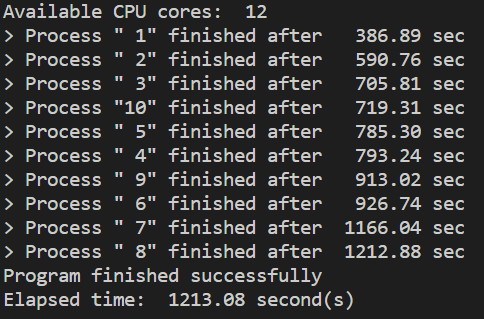
\includegraphics[scale=1]{ex6_results}

\includegraphics[scale=0.4]{ex6_stats_front}

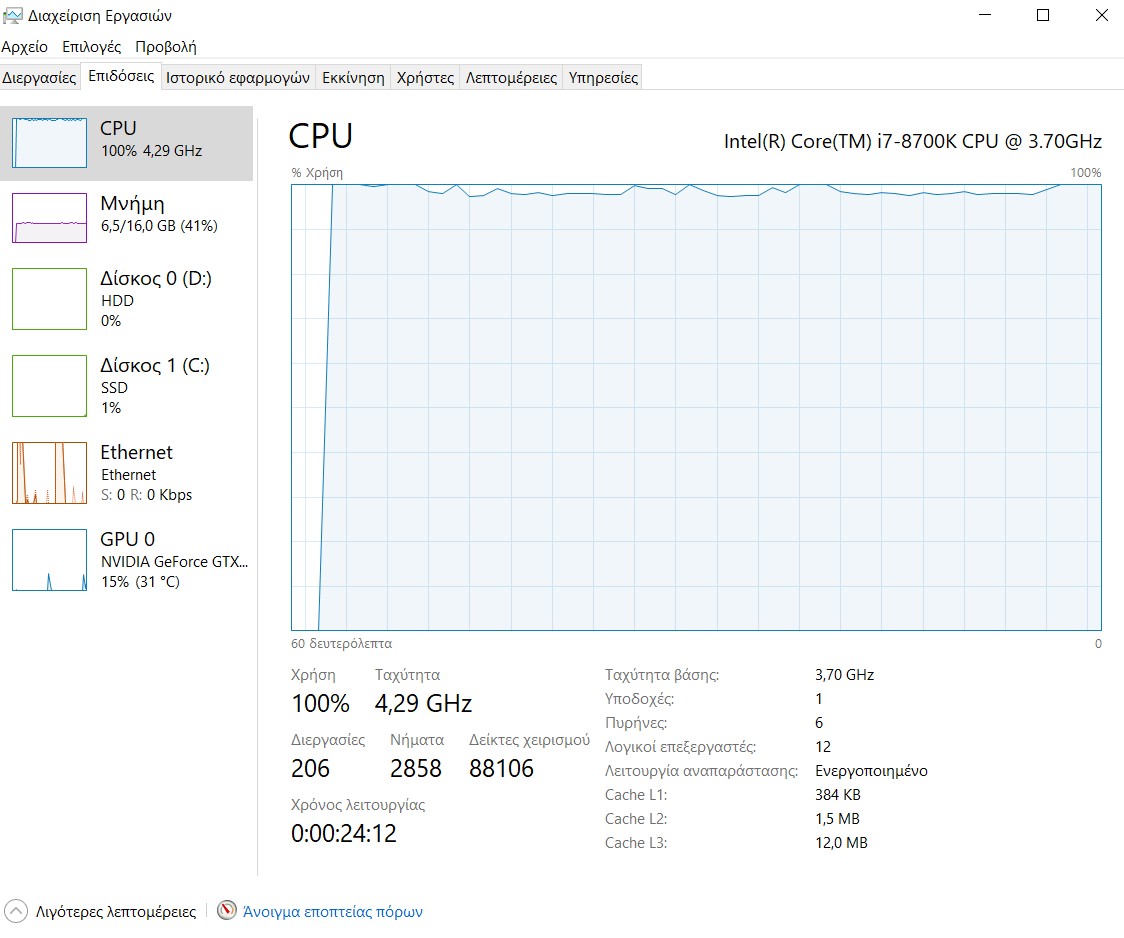
\includegraphics[scale=0.45]{ex6_stats_back}
\end{center}

\pagebreak

\section*{Άσκηση 7 (9.18)}

Έστω η συνάρτηση $\mathcal{P}(n) = (\vec{p},\:\vec{\alpha})$, 
όπου $\vec{p} \in \mathbb{P}^{k}$ και 
$\vec{\alpha} \in \mathbb{N}^{*k}$, $k \in \mathbb{N}^{*}$ 
εκφράζουν την παραγοντοποίηση του $n$ σε πρώτους, δηλαδή:
\[
	n\; =\; \prod_{i = 1}^{k}p_{i}^{\alpha_{i}}
\]
\[
	p_i \neq p_j\; \forall i \neq j
\]
\[
	p_i \in \mathbb{P},\;\; \alpha_{i} \in \mathbb{N^{*}}
\]

\vspace{0.1in}
\noindent
Αυτό ακριβώς υλοποιεί η συνάρτηση 
\texttt{\lt prime\_factorization(n:int)} (αλγόριθμος
δοκιμαστικής διαίρεσης). Προκύπτει γρήγορα απάντηση για τους 
ακεραίους {\lt 6553130926752006031481761} και
\texttt{9999109081} 
καθώς όλοι οι πρώτοι παράγοντές τους είναι μικροί.\\ 

\vspace{0.1in}
\noindent
Σύμφωνα με το κριτήριο {\lt Korselt}, για κάθε έναν από αυτούς 
τους πρέπει να ισχύει:
\begin{itemize}
	\item $a_i = 1$ για κάθε $1 \leq i \leq k$
	\item $p_i - 1 \mid n - 1$ για κάθε $1 \leq i \leq k$
\end{itemize}
Οι δοσμένοι ακέραιοι πληρούν τα παραπάνω κριτήρια. \\

\vspace{0.1in}
\noindent
(Υλοποίηση: \textbf{κώδικας/{\lt ex7/ex7.py}})


\section*{Άσκηση 8 (9.28)}

Οι ακέραιοι $835335 \cdot 2^{39014} \pm 1$ περνούν το τεστ του {\lt Fermat}.
\begin{itemize}
	\item $\mathbf{n_1 = 835335 \cdot 2^{39014} + 1}$: Ψευδοπρώτος ως προς τη βάση $a_1 \in \ints,\;\; a_1 \approx 2^{39033.011512}$
	\item $\mathbf{n_2 = 835335 \cdot 2^{39014} - 1}$: Ψευδοπρώτος ως προς τη βάση $a_2 \in \ints,\;\; a_2 \approx 2^{39033.632355}$
\end{itemize}
Οι $a_1$ και $a_2$ είναι τυπωμένοι αναλυτικά στα αρχεία \texttt{\lt n1.txt} και \texttt{\lt n2.txt} 
αντίστοιχα.

{ \lt
\begin{verbatim}
n1 is probable prime with respect 2^39033.011512 (elapsed: 84.548 sec)
n2 is probable prime with respect 2^39033.632355 (elapsed: 166.835 sec)
\end{verbatim}
}

\vspace{0.1in}
\noindent
(Υλοποίηση: \textbf{κώδικας/{\lt ex8/ex8.py}})


\section*{Άσκηση 9 (10.1)}
Ο αλγόριθμος δοκιμαστικής διαίρεσης εξάγει τα παρακάτω 
αποτελέσματα:
\[
	\mathbf{2^{62} - 1}\; =\; 3 \cdot 715827883 
	\cdot 2147483647
\]
\[
	\mathbf{2^{102} - 1}\; =\; 3^{2} \cdot 7 \cdot 103 
	\cdot 307 \cdot 2143 \cdot 2857 \cdot 6529 
	\cdot 11119 \cdot 43691 \cdot 131071
\]

\vspace{0.1in}
\noindent
(Υλοποίηση: \textbf{κώδικας/{\lt ex9/ex9.py}})

\pagebreak

\section*{Άσκηση 10 (10.8)}

\noindent
Το πρόγραμμα επιλέγει 1000 τυχαίους ακεραίους των {\lt 100 bits}, δηλαδή:
{ \large
\[
	n_i \xleftarrow{\$} [2^{99},\:2^{100}) \cap \ints,\;\; i \in \{1,\:2,\:...,\:1000\}
\]
}

\noindent
Η συνάρτηση \texttt{\lt lehman(int, float)} έχει δυο παραμέτρους 
εισόδου: τον αριθμό προς παραγοντοποιηση, $\mathbf{n}$ και ένα 
χρονικό όριο σε δευτερόλεπτα (ίσο με $10$ στη 
συγκεκριμένη άσκηση). Ως αποτέλεσμα επιστρέφει έναν 
παράγοντα $\mathbf{f}$ του $n$. Ο αλγόριθμος είναι επιτυχής άν 
\begin{enumerate}
\item τερματίσει πριν το χρονικό όριο και επιπλέον
\item $f \neq 1\:\vee\: f \neq n\:\vee\: f \in \ints$ (δεν έχει τιμή {\lt None})
\end{enumerate}
Συνολικά, βρέθηκε παράγοντας για 16 ακεραίους. Ενδεικτικά:
\begin{itemize}
	\item $n_{21} = 674.902.139.001.917.536.149.940.578.006\;$ με $\;1.739.779.667.412.498\:|\:n_{21}$
	\item $n_{31} = 876.328.564.129.523.250.183.808.043.827\;$ με $\;29.891.192.611.171\:|\:n_{31}$
	\item $n_{551} = 949.629.530.912.133.951.962.690.604.832\;$ με $\;49.596.489.117.889.648\:|\:n_{551}$
\end{itemize}

\noindent
Τα αποτελέσματα αναγράφονται αναλυτικά στο αρχείο \textbf{\lt ``results.txt"}.

{ \lt
\begin{verbatim}
Produced a factor for   1.600% of integers (16 / 1000)
Elapsed time: 1641.572 sec
\end{verbatim}
}

\vspace{0.1in}
\noindent
(Υλοποίηση: \textbf{κώδικας/{\lt ex10/ex10.py}})

\section*{Άσκηση 11 (10.21)}

Η υλοποίηση που έγινε για τον {\lt Pollard-}ρ στη συγκεκριμένη άσκηση στοχεύει στην εύρεση ενός παράγοντα του ακεραίου $N$ (μοναδική παράμετρος). Ισχύουν οι αρχικοποιήσεις:
\begin{itemize}
	\item $F(x) = (x^2 + 1)\:mod\:N$
	\item $X_0 \xleftarrow{\$} \{2,\:3,\:...,\:N-1\}$
	\item $X \coloneqq X_0$
	\item $Y \coloneqq X_0$
\end{itemize}

\noindent
Ο αλγόριθμος τερματίζει όταν $1 < d < N$ και ο $d$ επιστρέφεται ως αποτέλεσμα, 
όπου \\ 
$d = gcd(\vert X - Y \vert,\:N)$. \\

\noindent
Για $\mathbf{N = 2^{257} - 1}$ και αρχικοποιώντας το σπόρο της γεννήτριας της {\lt Python} με $s = 42$, λαμβάνονται τα ακόλουθα αποτελέσματα:

{ \lt
\begin{verbatim}
Found non-trivial factor: 535006138814359
Elapsed time: 70.564 sec
Execution steps: 17571888
\end{verbatim}
}

\vspace{0.1in}
\noindent
(Υλοποίηση: \textbf{κώδικας/{\lt ex11/ex11.py}})

\pagebreak

\section*{Άσκηση 12 (11.3)}

Για τη λύση της άσκησης χρησιμοποιήθηκαν:
\begin{enumerate}
	\item \textbf{Συνάρτηση Δοκιμαστικής Διαίρεσης:} Όπως και στις προηγούμενες ασκήσεις.
	\item \textbf{Συνάρτηση {\lt Euler}:} Για $n = p_1^{a_1} \cdot p_2^{a_2} \cdot ... \cdot p_k^{a_k}$, επιστρέφει:
	\[
		\phi(n) = n \prod_{i=1}^{k}\left(1 - \frac{1}{p_i}\right)
	\]
	ή ισοδύναμα, για την αποφυγή χρήσης αριθμών κινητής υποδιαστολής:
	\[
		\phi(n) = \Phi_{k+1}(n)
	\]
	\[
		\Phi_{i}(n) = 
		\left\{
		\begin{array}{ll}
			\Phi_{i-1}(n) - \lfloor \frac{\Phi_{i-1}(n)}{p_{i-1}} \rfloor 
			& \text{για } i \geq 2 \\
			n & \text{για } i = 1
		\end{array}
		\right.
	\]
	\item \textbf{Αλγόριθμος Υπολογισμού Ιδιωτικού Κλειδιού:} Για είσοδο $pk = (e,\:N)$, επιστρέφει $sk = (d,\:N)$ με $e \cdot d \equiv 1\:(mod\:\phi(N))$.
	\item \textbf{Αλγόριθμος {\lt RSA}:} Για είσοδο το κρυπτοκείμενο και το $sk$, επιστρέφει το αποκρυπτογραφημένο μήνυμα.
\end{enumerate}

\hfill

\noindent
Αρχικά, έχουμε $pk = (19,\:11413)$ και άρα υπολογίζουμε $sk = (1179,\:11413)$. Έτσι, για:
\begin{align*}
	C = (&3203, 909, 3143, 5255, 5343,
    3203, 909, 9958, 5278, 5343, 
    9958, 5278, \\
    &4674, 909, 9958,
    792, 909, 4132, 3143, 9958,
    3203, 5343, 792, 3143, 4443)
\end{align*}
τότε η κλήση της συνάρτησης \texttt{\lt RSA(sk, C)} επιστρέφει:
\begin{align*}
M = (&119, 101, 108, 99, 111, 119, 101, 32, 116, 111, 32, 116, \\
&104, 101, 32, 114, 101, 97, 108, 32, 119, 111, 114, 108, 100)
\end{align*}
Του οποίου η αποκωδικοποίηση σε χαρακτήρες {\lt ASCII} είναι:
{ \lt
\begin{center}
	``\textbf{welcowe to the real world}"
\end{center}
}

\hfill

\vspace{0.3in}
\noindent
(Υλοποίηση: \textbf{κώδικας/{\lt ex12/ex12.py}})

\pagebreak

\section*{Άσκηση 13 (12.2)}

Για είσοδο $pk = (e,\:N) = (50736902528669041,\:194749497518847283)$ δίνονται τα βήματα 
της επίθεσης του {\lt Wiener}:
\begin{enumerate}
	\item Αποθηκεύουμε σε μια λίστα, A, το συνεχές κλάσμα του $\frac{e}{N}$ με ακρίβεια 40 συντελεστών:
	\begin{align*}
	\frac{e}{N} = [&0;\:3, 1, 5, 5, 3, 2, 1, 1, 2, 1, 2, 1, 1, 1, 2, 1, 4, 1, 26, 4, \\
	&2, 3, 1, 18, 10, 6, 3, 180, 2, 2, 1, 1, 4, 2, 5, 1, 2, 3, 83, 9]
	\end{align*}
	\item Για κάθε $i \in [1,\:40]$ αποθηκεύουμε σε μια λίστα, {\lt F}, τους πραγματικούς αριθμούς 
	$x_i$, όπου $x_i = [A_0;\:A_1, ..., A_i]$
	\item Για κάθε $i \in [1,\:40]$ χρησιμοποιούμε την κλάση \texttt{\lt fractions.Fraction} για 
	να μας επιστρέψει τους ακεραίους $N_i$ και $D_i$, όπου $\frac{N_i}{D_i}$ το ανάγωγο κλάσμα του 
	$x_i$. Στην επανάληψη για $i = 12$ ισχύει $x_{12} \approx 0.260523921268139$, άρα 
	$(N_{12},\:D_{12}) = (5440,\:20881)$.
	\item Ισχύει ότι $\mathbf{2^{e \cdot D_{12}} \equiv 2(mod\:N)}$, επομένως επιστρέφεται το 
	$D_{12} = 20881$ ως πιθανό ιδιωτικό κλειδί.
\end{enumerate}

\noindent
Εισάγοντας το \href{https://github.com/drazioti/book_crypto/blob/master/public_key_crypto/7.2}{κρυπτοκείμενο} σε έναν \href{https://www.base64decode.org/}{αποκωδικοποιητή {\lt Base64}} προκύπτει 
μια λίστα {\lt Python}:
\[
C=[47406263192693509,51065178201172223, ..., 134434295894803806,57208077766585306]
\]
Είσάγοντας το $sk = (D_{12},\:N)$ και το $C$ στον {\lt RSA} προκύπτει μια λίστα ακεραίων των 
οποίων η κωδικοποίηση σε χαρακτήρες {\lt ASCII} είναι:

{\lt
\begin{center}
	``\textbf{ Just because you are a character doesn't mean that you have character}"
\end{center}
}
\vspace{0.1in}
\noindent
(Υλοποίηση: \textbf{κώδικας/{\lt ex13/ex13.py}})

\section*{Άσκηση 14 (13.2)}

Για $N = 899,\;e = 839,\;m = 3,\; s = 301\; \Rightarrow\; \mathbf{a = s^{e}\:mod\:N = 675} \neq m$, 
άρα η ψηφιακή υπογραφή $s$ είναι λάθος.

\vspace{0.3in}
\noindent
(Υλοποίηση: \textbf{κώδικας/{\lt ex14/ex14.py}})

\end{document}